\documentclass{article} 

\usepackage{amsmath,amsthm,graphicx}
\usepackage{amsfonts}
\usepackage{amssymb}
\usepackage{mathtools,array}
\usepackage{tikz}
\usepackage{tkz-euclide}
\usepackage{multicol}
\usepackage{enumerate}
\usepackage{datetime}
\newdate{date}{20}{01}{2015}

\graphicspath{ {F:/repos/mcgill/MATH223/Assignments/} }

\usetkzobj{all}
\usetikzlibrary{calc,positioning,intersections,quotes,decorations.markings}

\newtheorem{problem}{Problem} 
\theoremstyle{definition} 
\newtheorem*{solution}{Solution} 

\setlength\parskip{\baselineskip}
\setlength\parindent{0pt}

\begin{document} \title{Assignment 1} 

\author{Yang David Zhou, ID 260517397} 
\date{\displaydate{date}}
\maketitle

\begin{problem} Proofs.

\end{problem}

\begin{solution}

(a) \begin{proof}
The Pythagorean theorem states that in a right triangle where $c$ is the length of the hypotenuse and $a,b$ are the lengths of the other two sides, the formula $c^2=a^2+b^2$ is true.

In general, any non-right triangle can be divided into two right angled triangles by dropping a vertical from a vertex that is perpendicular to the opposite edge, like in the diagram below.

\begin{center}
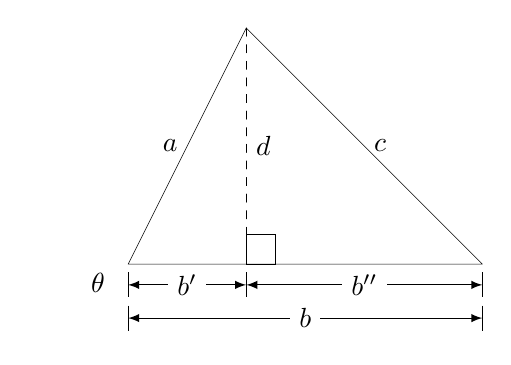
\begin{tikzpicture}[scale=1.5]
\tkzDefPoint(3,0){A}
\tkzDefPoint(0,0){C}
\tkzDefPoint(1,2){B}
\tkzDefPoint(1,0){D}
\tkzDrawPolygon(A,B,C)
\tkzDrawSegment[dashed](B,D)
\tkzLabelAngle[pos=0.3](B,C,A){$\theta$}
\tkzMarkRightAngle(B,D,A)
\tkzLabelSegment[right](B,D){$d$}
\tkzLabelSegment[right](B,A){$c$}
\tkzLabelSegment[left](C,B){$a$}
\foreach \Nodo in {A,D}
 \draw ([yshift=-2pt]\Nodo) -- ([yshift=-8pt]\Nodo);
\draw[<->,>=latex] ([yshift=-5pt]A) -- node[fill=white] {$b''$} ([yshift=-5pt]D);
\foreach \Nodo in {C,D}
 \draw ([yshift=-2pt]\Nodo) -- ([yshift=-8pt]\Nodo);
\draw[<->,>=latex] ([yshift=-5pt]C) -- node[fill=white] {$b'$} ([yshift=-5pt]D);
\foreach \Nodo in {A,C}
 \draw ([yshift=-10pt]\Nodo) -- ([yshift=-16pt]\Nodo);
\draw[<->,>=latex] ([yshift=-13pt]A) -- node[fill=white] {$b$} ([yshift=-13pt]C);
\end{tikzpicture}
\end{center}

Define $b=b'+b''$ (1).

Which can be rearranged, $b''=(b-b')$ (2).

By trigonometry we have $b'=a\cos \theta$ (3).

By the Pythagorean we have $a^2=d^2+(b')^2$ (4) and $c^2=d^2+(b'')^2$ (5).

Rearrange (4) and (5) for $d^2$ then set them equal,
\begin{align*}
c^2-(b'')^2&=a^2-(b')^2 \\
c^2&=a^2-(b')^2+(b'')^2 \\
&=a^2-(b')^2+(b-b')^2 \quad \text{By (2)} \\
&=a^2-(a\cos \theta )^2+(b-a\cos \theta)^2 \quad \text{By (3)} \\
&=a^2-a^2\cos ^2\theta+b^2-2ab\cos\theta+a^2\cos^2\theta \\
c^2&=a^2+b^2-2ab\cos\theta
\end{align*}

And we are done.
\end{proof}

(b) \begin{proof}
Geometrically, $v$ and $w$ form a plane and $u=v-w$ is a vector on that plane.
Together, $u,v,w$ form a triangle.
So we apply the Law of Cosines.

Define $\theta$ to be the angle opposite $u=v-w$.
By definition of the angle between two vectors, $\cos\theta=\frac{v\cdot w}{\|v\|\|w\|}$.
\begin{align*}
\|v-w\|^2&=\|v\|^2+\|w\|^2-2\|v\|\|w\|\cos\theta \\
\|v-w\|^2&=\|v\|^2+\|w\|^2-2\|v\|\|w\|\left(\frac{v\cdot w}{\|v\|\|w\|}\right) \quad \text{By definition} \\
\|v-w\|^2&=\|v\|^2+\|w\|^2-2v\cdot w \\
2v\cdot w&=\|v\|^2+\|w\|^2-\|v-w\|^2 \\
2v\cdot w&=\|v\|^2+\|w\|^2-(\|v\|^2+\|w\|^2-2\|v\|\|w\|\cos\theta) \\
2v\cdot w&=2\|v\|\|w\|\cos\theta \\
v\cdot w&=\|v\|\|w\|\cos\theta \\
\end{align*}

And we are done.
\end{proof}

\end{solution}

\begin{problem} 

Complex numbers.

\end{problem}

\begin{solution}

(a) \begin{align*}
\frac{1}{2}(z+\tilde{z})&=\frac{1}{2}((a+bi)+(a-bi)) \\
&=\frac{1}{2}(a+a+bi-bi) \\
&=\frac{1}{2}(2a) \\
&=a
\end{align*}

(b) \begin{align*}
\frac{1}{2i}(z-\tilde{z})&=\frac{1}{2i}((a+bi)-(a-bi)) \\
&=\frac{1}{2i}(a+bi-a+bi) \\
&=\frac{1}{2i}(2bi) \\
&=b
\end{align*}

(c) 
\begin{multicols}{2}
Case $z=0$: 
\begin{align*}
zw&=0 \\
z&=\frac{0}{(a+bi)} \\
&=0
\end{align*}
Case $w=0$:
\begin{align*}
zw&=0 \\
w&=\frac{0}{(a+bi)} \\
&=0
\end{align*}
\end{multicols}

\end{solution}

\begin{problem} 

Matrix multiplication.

\end{problem}

\begin{solution}

In order for the product of two matrices $M=AB$ to be valid, the number of columns in $A$ must equal the number of rows in $B$.
Otherwise the product is not well defined.

Only $ABC,BCA,CAB$ will yield valid products.

\begin{align*}
ABC&=
\begin{bmatrix}
1 & 0 & -i \\
-1 & i & 0 \\
0 & 0 & 1
\end{bmatrix}
\begin{bmatrix}
i & 0 \\
0 & -i \\
1 & 0
\end{bmatrix} C =
\begin{bmatrix}
(i+0-i) & (0+0+0) \\
(-i+0+0) & (0+1+0) \\
(0+0+1) & (0+0+0)
\end{bmatrix} C \\
&=
\begin{bmatrix}
0 & 0 \\
-i & 1 \\
1 & 0
\end{bmatrix}
\begin{bmatrix}
-1 & 1 & 2 \\
i & 2i & i
\end{bmatrix} =
\begin{bmatrix}
(0+0) & (0+0) & (0+0) \\
(-i+i) & (i+2i) & (2i+i) \\
(-1+0) & (1+0) & (2+0)
\end{bmatrix} \\
&=
\boxed{
\begin{bmatrix}
0 & 0&0\\
0&3i&3i\\
-1&1&2
\end{bmatrix}}
\end{align*}

\begin{align*}
BCA&=
\begin{bmatrix}
i & 0 \\
0 & -i \\
1 & 0
\end{bmatrix}
\begin{bmatrix}
-1 & 1 & 2 \\
i & 2i & i
\end{bmatrix} A =
\begin{bmatrix}
(-i+0) & (i+0) & (2i+0) \\
(0+1) & (0+2) & (0+1) \\
(-1+0) & (1+0) & (2+0)
\end{bmatrix} A \\
&=
\begin{bmatrix}
-i & i & 2i \\
1&2&1\\
-1&1&2
\end{bmatrix}
\begin{bmatrix}
1 & 0 & -i \\
-1 & i & 0 \\
0 & 0 & 1
\end{bmatrix} =
\begin{bmatrix}
(-i-i+0)&(0-1+0)&(-1+0+2i)\\
(1-2+0)&(0+2i+0)&(-i+0+1)\\
(-1-1+0)&(0+i+0)&(i+0+2)
\end{bmatrix} \\
&=
\boxed{
\begin{bmatrix}
-2i&-1&(-1+2i)\\
-1&2i&(1-i)\\
-2&i&(2+i)
\end{bmatrix}}
\end{align*}

\begin{align*}
CAB&=
\begin{bmatrix}
-1 & 1 & 2 \\
i & 2i & i
\end{bmatrix}
\begin{bmatrix}
1 & 0 & -i \\
-1 & i & 0 \\
0 & 0 & 1
\end{bmatrix} B =
\begin{bmatrix}
(-1-1+0)&(0+i+0)&(i+0+2)\\
(i-2i+0)&(0-2+0)&(1+0+i)
\end{bmatrix} B \\
&=
\begin{bmatrix}
-2&i&(2+i)\\
-i&-2&(1+i)
\end{bmatrix}
\begin{bmatrix}
i & 0 \\
0 & -i \\
1 & 0
\end{bmatrix} =
\begin{bmatrix}
(-2i+0+(2+i))&(0+1+0)\\
(1+0+(1+i))&(0+2i+0)
\end{bmatrix} \\
&=
\boxed{
\begin{bmatrix}
(2-i)&1\\
(2+i)&2i
\end{bmatrix}}
\end{align*}

\end{solution}

\begin{problem}

Row-reduced echelon form.

\end{problem}

\begin{solution}

My work for this is attached.
Shown below is only the final result.

\[
A=
\begin{bmatrix}
1&2&3&-1\\
2&3&0&1\\
1&1&-3&2
\end{bmatrix}\sim
\begin{bmatrix}
1&0&-9&5\\
0&1&6&-3\\
0&0&0&0
\end{bmatrix}
\]
\[
B=
\begin{bmatrix}
0&1&3\\
2&1&1\\
1&0&1
\end{bmatrix}\sim
\begin{bmatrix}
1&0&0\\
0&1&0\\
0&0&1
\end{bmatrix}
\]

\end{solution}

\begin{problem} 

Inverting matrices.

\end{problem}

\begin{solution}

My work for this is attached.
Shown below is only the final result.

\[
A^{-1}=
\begin{bmatrix}
0&-1&0&1\\
1&-4&-3&4\\
0&1&1&-1\\
0&-2&-3&3
\end{bmatrix}\]

\end{solution}

\begin{problem}

Linear combinations in a vector space.

\end{problem}

\begin{solution}

$M_{2,2}$ is clearly a vector space and a subspace of a vector space is also a vector space.
This subspace must then be closed under addition and multiplication so a linear combination of any two vectors in the space is also in this space.

$I^2$ can be shown to be a linear combination as follows,
\begin{align*}
I^2=\begin{bmatrix}
1&0\\0&1
\end{bmatrix}&=-2
\begin{bmatrix}
2&10\\
10&12
\end{bmatrix}+5
\begin{bmatrix}
1&4\\
4&5
\end{bmatrix}\\
&=
\begin{bmatrix}
-4&-20\\
-20&-24
\end{bmatrix}+
\begin{bmatrix}
5&20\\
20&25
\end{bmatrix}\\
&=
\begin{bmatrix}
1&0\\0&1
\end{bmatrix}
\end{align*}

I arrived at this solution by guessing and checking multiples of $10$ and $4$ that add up to $0$.

\end{solution}

\begin{problem} 

Validity of subspace.

\end{problem}

\begin{solution}

$W$ is clearly a subset of $\mathbb{R}^3$.

The zero vector $(0,0,0)$ is in $W$.
So, $a=0,b=0,c=0$.
\begin{enumerate}[a)]
 \item $0=3(0)$
 \item $0\leq 0\leq 0$
 \item $(0)(0)=0$
 \item $0=(0)^2$
\end{enumerate}

$u,v\in W\quad a,b\in \mathbb{R}$

\begin{multicols}{2}
$u=(u_1,u_2,u_3)$ with 
\begin{enumerate}[a)]
 \item $u_1=3u_2$
 \item $u_1\leq u_2\leq u_3$
 \item $u_1u_2=0$
 \item $u_2=u_1^2$
\end{enumerate}

$v=(v_1,v_2,v_3)$ with 
\begin{enumerate}[a)]
 \item $v_1=3v_2$
 \item $v_1\leq v_2\leq v_3$
 \item $v_1v_2=0$
 \item $v_2=v_1^2$
\end{enumerate}
\end{multicols}

\begin{align*}
z=(z_1,z_2,z_3)&=au+bv \\
&=(au_1+bv_1,au_2+bv_2,au_3+bv_3)
\end{align*}

(a) is a valid vector space constraint.
The argument for (a) is that both $u_1=3u_2$ and $v_1=3v_2$.
So for any $u,v,z\in W$,
\begin{align*}
z_1&=au_1+bv_1\\
&=a(3u_2)+b(3v_2)\\
&=3(au_2+bv_2)\\
&=3z_2
\end{align*}
And so (a) holds for addition and scalar multiplication.

(b) is not a valid vector space constraint.

The argument for (b) is that if $u_1\leq u_2$ then $au_1\leq au_2$.

Similarly, $bv_1\leq bv_2$.

But if $a<0$ and $b\geq 0$ then $|a|u_1\geq |a|u_2$.

Then there is no guarantee that $au_1+bv_2\leq au_2+bv_2$ is true.

The case where $b<0$ and $a\geq 0$ is true by symmetry.

A simple counter example would be $(0,0,0)+(-1)(0,0,1)=(0,0,-1)$.
Clearly $(0,0,-1)\notin W$.

And so $W$ is not closed under addition and scalar multiplication.
Therefore $W$ is not a vector space.

\end{solution}

\begin{problem} 

The union of two subspaces.

\end{problem}

\begin{solution}

\begin{proof}
Take the contrapositive to show that if neither $U\subseteq W$ nor $W\subseteq U$ then $U\cup W$ is not a subspace.

Choose two vectors $u,w$ such that $u\in U, u\notin W$ and $w\in W, w\notin U$.
So, $u,w\in U\cup W$.
Assume $U\cup W$ is a subspace.
So, $z=au+bw, z\in U\cup W$ which means $z\in U$ or $z\in W$.

Case $z\in U$:

$U$ is a vector space so if $u\in U$, then $(-a)u\in U$.
So, $z+(-a)u$ should also be in $U$.
\begin{align*}
z+(-a)u&=au+bw-au\\
&=bw
\end{align*}
But $w\notin U$ so $bw\notin U$. Contradiction.

The case where $z\in W$ is true by symmetry.
\end{proof}

\end{solution}

\end{document}